\documentclass[a4paper]{article}

\usepackage[utf8]{inputenc}  
\usepackage[francais]{babel}  
\usepackage[top=2cm, bottom=2cm, left=2cm, right=2cm]{geometry}
\usepackage{graphicx}

\begin{document}

\begin{titlepage}
	~ 
	\vfill
	\begin{center}
		\begin{Huge}
			Projet Administration Réseau : \\ Mise en pratique\\
		\end{Huge}
	\vfill
		\textbf{Hexanôme 4211 :} 
			\\Sandra \bsc{Mondain}, Elisa \bsc{Abidh}, 
			\\Gaël \bsc{Motte}, Armand \bsc{Rossius}, 
			\\Nicolas \bsc{Silva}, Julien \bsc{Levesy}\\
	\vfill
	\end{center}
	\vfill
\end{titlepage}


\section{Configuration de Nagios}

cf. fichiers de configurations fournis conjointement à ce livrable.

\section{Analyse critique}
Nagios permet, une fois installé et configuré, de surveiller l'activité d'une ou plusieurs machines de façon relativement autonôme puisque le logiciel est à même de notifier l'administrateur en cas de problème. Ce type de fonctionnalité en fait un outil intéressant car il fournit une visibilité sur l'activité des systèmes surveillés, sans toutefois accaparer l'attention de l'administrateur. L'interface de visualisation étant basé sur un front-end web, il est possible d'accéder aux données de supervision à distance, ce qui est pimordial pour un administrateur. ~\\

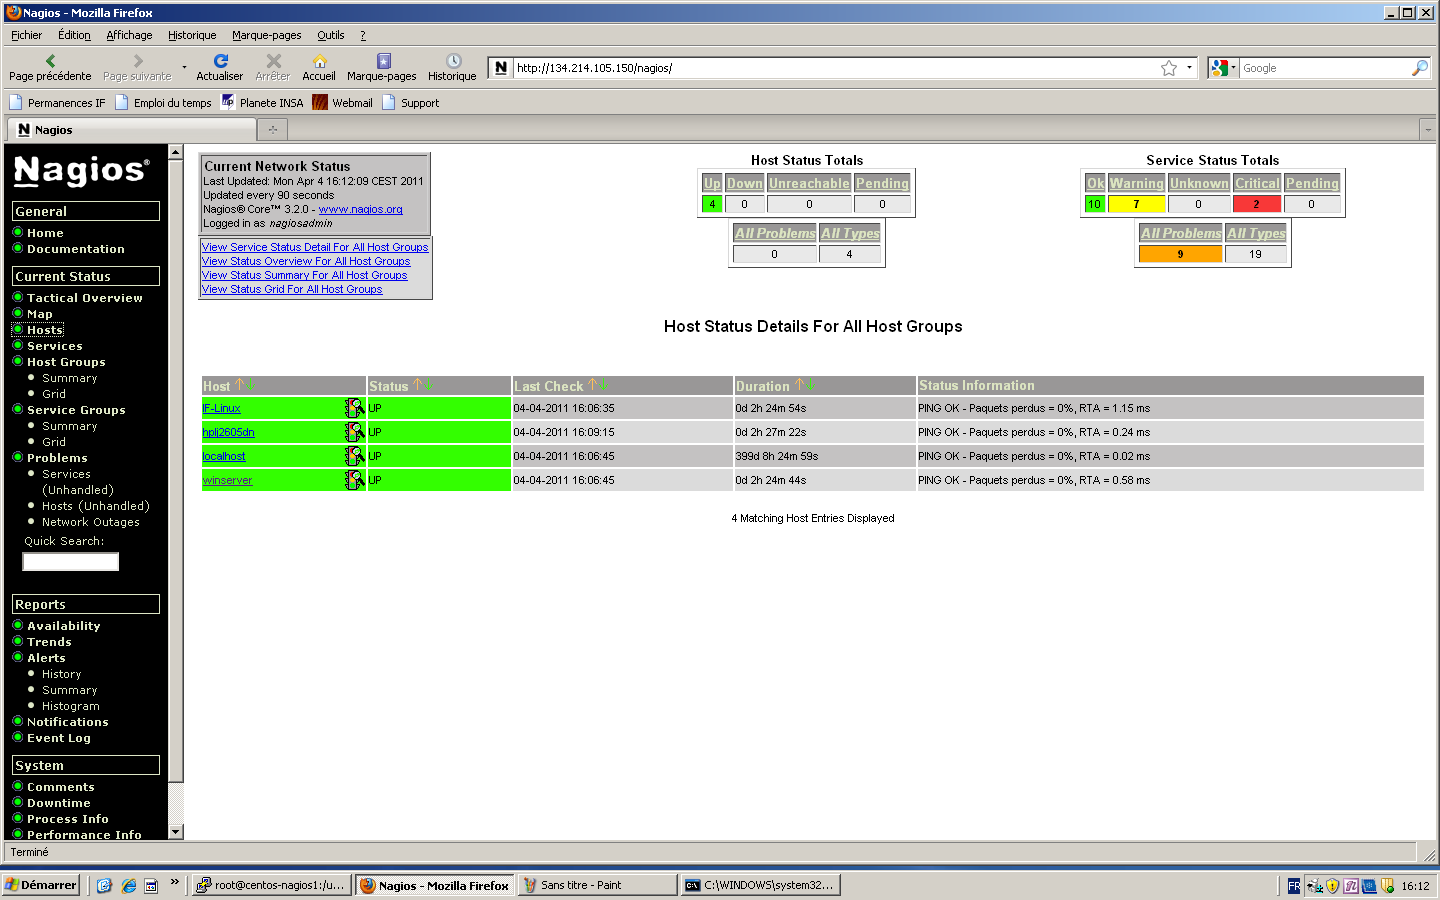
\includegraphics[width=\linewidth]{nagios-global.PNG}

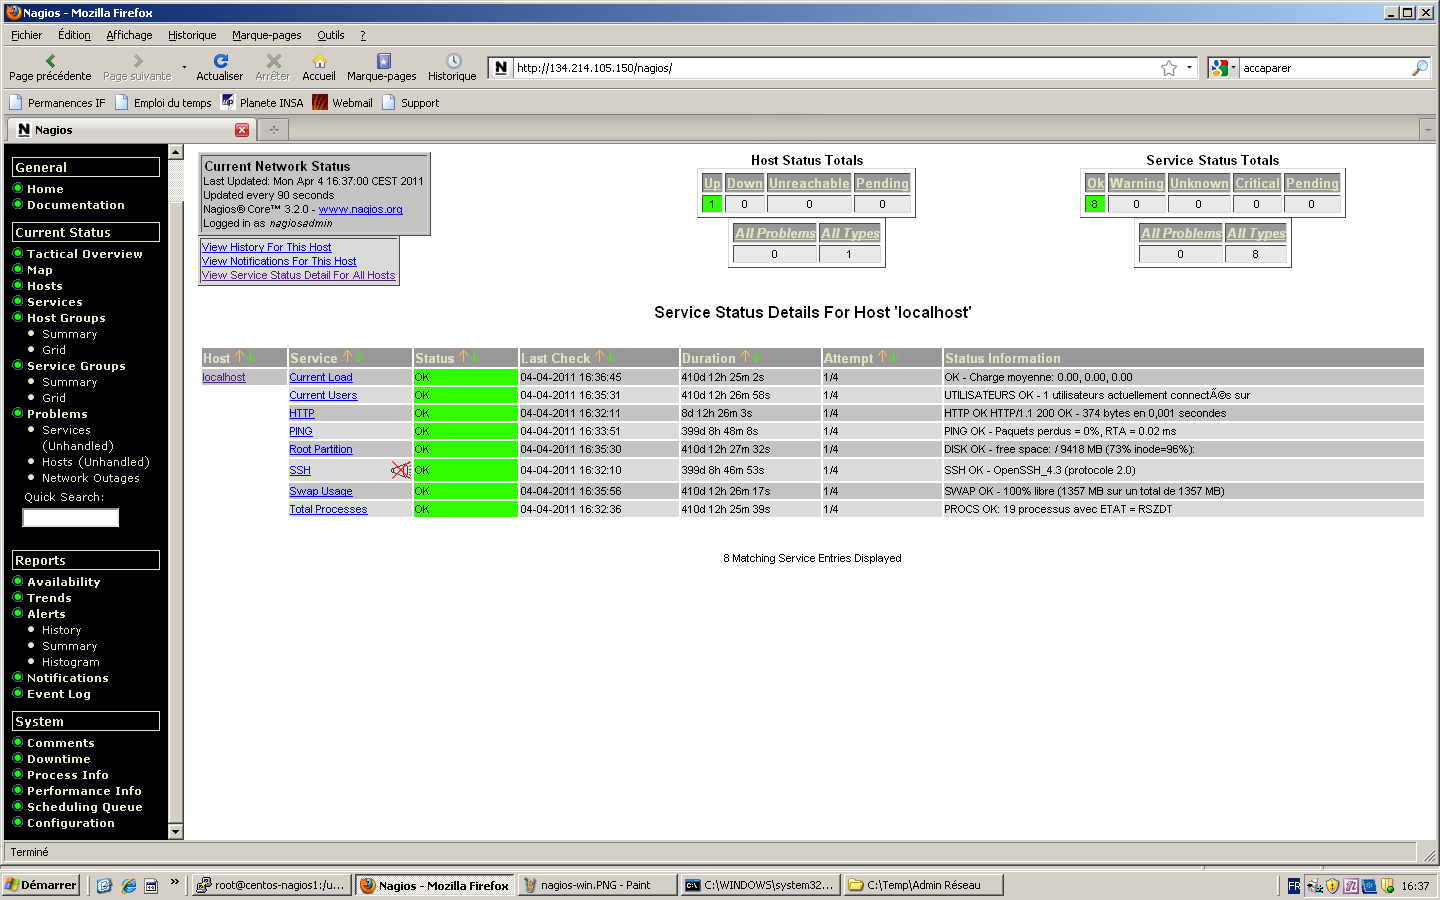
\includegraphics[width=\linewidth]{nagios-lin.PNG}

Nous pouvons voir en un coup d'oeil l'état de fonctionnement des mâchines supervisées, ainsi que l'état des différents services proposés par chaque machine. Ce niveau de détail permet de déterminer plus facilement les causes de dysfonctionnements, couplé avec un outil comme MRTG pour assurer la supervision réseau.

Nous regrettons cependant la difficulté de mise en place de la supervision avec Nagios, de par l'absence d'interface graphique pour la configuration. Il en résulte un outil utile, mais difficile d'accès, et donc coûteux en mise en fonctionnement et en maintenance.

Une fois installé l'interface web de Nagios est suffisament facile d'utilisation pour justifier les efforts liés à la configuration du logiciel.

Notons toutefois que les informations délivrées par Nagios ne sont pas toujours exacte, comme le montre cette capture attestant l'inactivité du processus explorer de windows alors que nous avons pu constater par nous même que l'explorer fonctionnait.  ~\\

% capture explorer
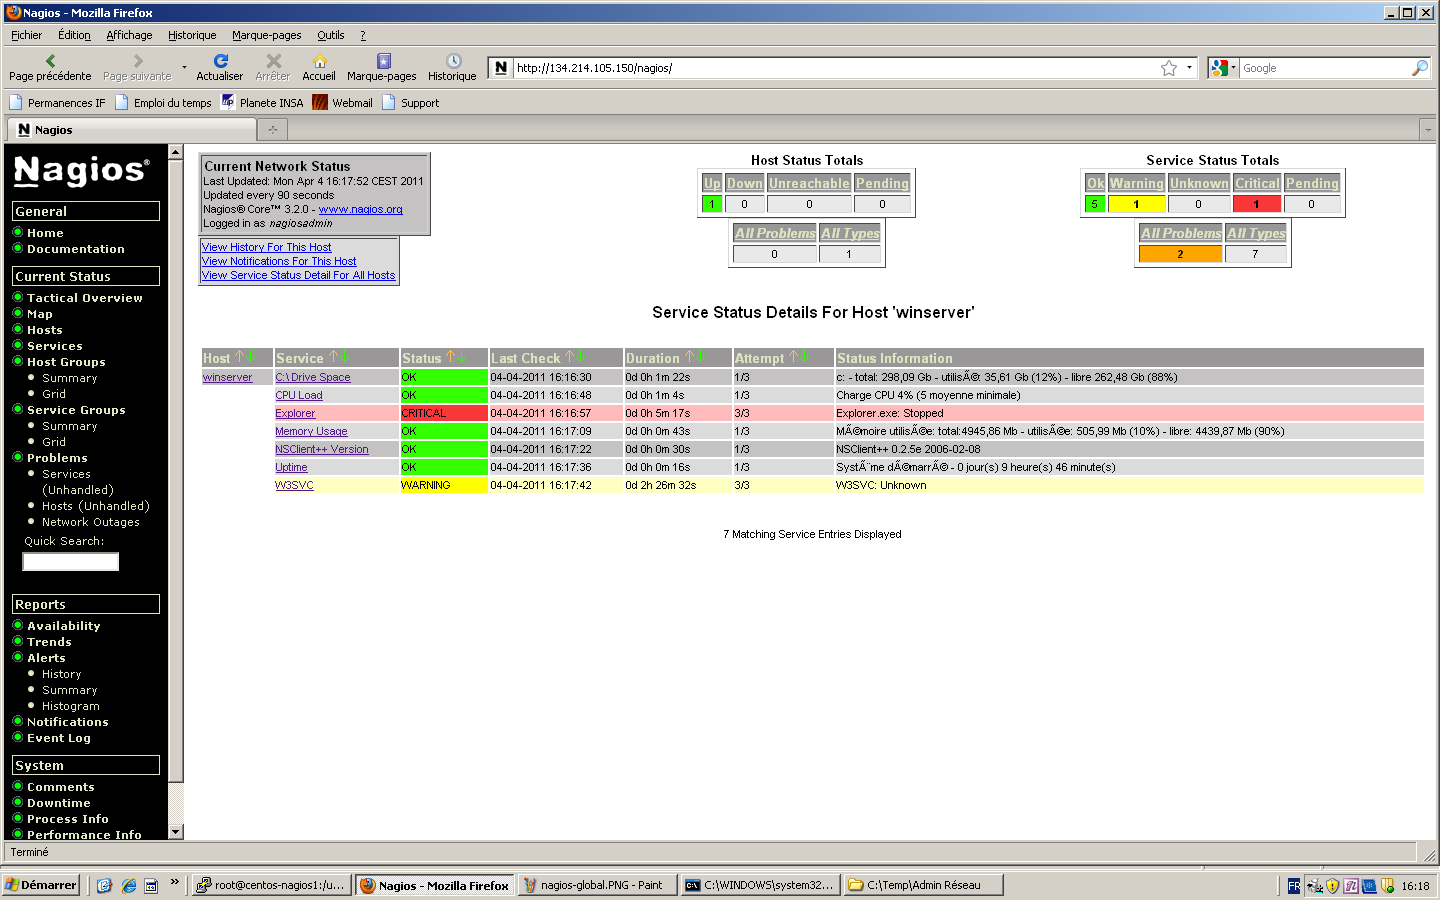
\includegraphics[width=0.7\linewidth]{nagios-win.PNG}

\end{document}
